% !TEX root = main.tex
\bibliography{literatur}
\bibliographystyle{babalpha}
\newpage
\listoffigures
\listoftables
\addcontentsline{toc}{section}{Attachments}
\section*{Attachments}
\setcounter{section}{6}
\newpage

\begin{table}[H]
    \centering
    \caption[Tabelle mit den jeweiligen $T_1$- und $T_2$-Zeiten in Abhängigkeit von der Konzentration dargestellt.]{ In der Tabelle werden die $T_1$- und $T_2$-Zeiten in Abhängigkeit von der jeweiligen Konzentration aufgetragen. Hierbei muss angemerkt werden, dass durch die jeweiligen Fits eine Unsicherheit ausgegeben wurde, diese aber sehr klein ist. Es ergibt also hier wenig Sinn diese noch explizit hinzu zu schreiben, da sonst die $T_1$/$T_1$-Zeiten teilweise mit sechs Nachkommastellen angegeben werden würden. Außerdem werden die Daten nur zur qualitativen Betrachtung in dem Kapitel \glqq 2D-MRI\grqq \, verwendet.}\label{tab:T1T2}
    \begin{tabular}{lll}
    \hline
    \multicolumn{1}{|l|}{}            & \multicolumn{1}{l|}{T1}      & \multicolumn{1}{l|}{T2}      \\ \hline
    \multicolumn{1}{|l|}{\ce{Cu2+}    $\SI{250}{\micro\mole}$}  & \multicolumn{1}{l|}{1394,84} & \multicolumn{1}{l|}{1215,51} \\ \hline
    \multicolumn{1}{|l|}{\ce{Cu2+}    $\SI{500}{\micro\mole}$}  & \multicolumn{1}{l|}{1003,40}  & \multicolumn{1}{l|}{1066,44} \\ \hline
    \multicolumn{1}{|l|}{\ce{Cu2+}    $\SI{1000}{\micro\mole}$} & \multicolumn{1}{l|}{646,85} & \multicolumn{1}{l|}{748,40} \\ \hline
    \multicolumn{1}{|l|}{\ce{Cu2+}    $\SI{2000}{\micro\mole}$} & \multicolumn{1}{l|}{431,27} & \multicolumn{1}{l|}{341,83}  \\ \hline
                                      &                              &                              \\ \hline
    \multicolumn{1}{|l|}{\ce{Mn2+}    $\SI{25}{\micro\mole}$}     & \multicolumn{1}{l|}{1178,28} & \multicolumn{1}{l|}{548,34} \\ \hline
    \multicolumn{1}{|l|}{\ce{Mn2+}    $\SI{50}{\micro\mole}$}     & \multicolumn{1}{l|}{725,86} & \multicolumn{1}{l|}{279,86} \\ \hline
    \multicolumn{1}{|l|}{\ce{Mn2+}    $\SI{100}{\micro\mole}$}    & \multicolumn{1}{l|}{316,09} & \multicolumn{1}{l|}{170,99} \\ \hline
    \multicolumn{1}{|l|}{\ce{Mn2+}    $\SI{200}{\micro\mole}$}    & \multicolumn{1}{l|}{180,24} & \multicolumn{1}{l|}{69,15} \\ \hline
                                      &                              &                              \\ \hline
    \multicolumn{1}{|l|}{Wasser}      & \multicolumn{1}{l|}{2199,46} & \multicolumn{1}{l|}{1901,06} \\ \hline
    \end{tabular}
    \end{table}

% \begin{table}[H]
%     \centering
%     \caption{$T_1$ und $T_2$ abhängig vom Kontrastmittel und dessen Konzentration.}
%     \begin{tabular}{lllll}  \hline
%     \multicolumn{1}{|l||}{}            & \multicolumn{1}{l|}{T1 in \si{\milli \second}}      & \multicolumn{1}{l|}{U(T1)-Fit in \si{\milli \second}} & \multicolumn{1}{l|}{T2 in \si{\milli \second}}      & \multicolumn{1}{l|}{U(T2)-Fit in \si{\milli \second}}  \\ \hline
%     \multicolumn{1}{|l||}{Wasser}      & \multicolumn{1}{l|}{2199,46} & \multicolumn{1}{l|}{0,003027}  & \multicolumn{1}{l|}{1901,06} & \multicolumn{1}{l|}{89,83}      \\ \hline \hline
%     \multicolumn{1}{|l||}{\ce{Cu^2+}    ($\SI{0.5}{\frac{\mol}{\metre \tothe{3}}}$)}  & \multicolumn{1}{l|}{1394,84} & \multicolumn{1}{l|}{0,001055}  & \multicolumn{1}{l|}{1215,51} & \multicolumn{1}{l|}{0,0002529}  \\ \hline
%     \multicolumn{1}{|l||}{\ce{Cu^2+}    ($\SI{1.0}{\frac{\mol}{\metre \tothe{3}}}$)}  & \multicolumn{1}{l|}{1003,4}  & \multicolumn{1}{l|}{0,0004851} & \multicolumn{1}{l|}{1066,44} & \multicolumn{1}{l|}{0,0002621}  \\ \hline
%     \multicolumn{1}{|l||}{\ce{Cu^2+}    ($\SI{2.0}{\frac{\mol}{\metre \tothe{3}}}$)} & \multicolumn{1}{l|}{646,849} & \multicolumn{1}{l|}{71,54}     & \multicolumn{1}{l|}{748,404} & \multicolumn{1}{l|}{0,0001937}  \\ \hline
%     \multicolumn{1}{|l||}{\ce{Cu^2+}    ($\SI{4.0}{\frac{\mol}{\metre \tothe{3}}}$)} & \multicolumn{1}{l|}{431,268} & \multicolumn{1}{l|}{0,0002906} & \multicolumn{1}{l|}{341,83}  & \multicolumn{1}{l|}{0,0001228}  \\ \hline \hline
%     \multicolumn{1}{|l||}{\ce{Mn^2+}    ($\SI{0.05}{\frac{\mol}{\metre \tothe{3}}}$)}     & \multicolumn{1}{l|}{1178,28} & \multicolumn{1}{l|}{0,0009801} & \multicolumn{1}{l|}{548,337} & \multicolumn{1}{l|}{0,0001258}  \\ \hline
%     \multicolumn{1}{|l||}{\ce{Mn^2+}    ($\SI{0.10}{\frac{\mol}{\metre \tothe{3}}}$)}     & \multicolumn{1}{l|}{725,857} & \multicolumn{1}{l|}{0,0006027} & \multicolumn{1}{l|}{279,858} & \multicolumn{1}{l|}{0,00008179} \\ \hline
%     \multicolumn{1}{|l||}{\ce{Mn^2+}    ($\SI{0.20}{\frac{\mol}{\metre \tothe{3}}}$)}    & \multicolumn{1}{l|}{316,085} & \multicolumn{1}{l|}{0,0003079} & \multicolumn{1}{l|}{170,996} & \multicolumn{1}{l|}{0,0001182}  \\ \hline
%     \multicolumn{1}{|l||}{\ce{Mn^2+}    ($\SI{0.40}{\frac{\mol}{\metre \tothe{3}}}$)}    & \multicolumn{1}{l|}{180,244} & \multicolumn{1}{l|}{0,0001274} & \multicolumn{1}{l|}{69,1512} & \multicolumn{1}{l|}{0,0000547}  \\ \hline
%     \end{tabular}
%     \label{tab:T1T2Kontrast}
% \end{table}

\begin{figure}[H]
    \begin{subfigure}[b]{0.5\textwidth}
        \centering
        \resizebox{1\textwidth}{!}{% GNUPLOT: LaTeX picture with Postscript
\begingroup
  % Encoding inside the plot.  In the header of your document, this encoding
  % should to defined, e.g., by using
  % \usepackage[cp1252,<other encodings>]{inputenc}
  \inputencoding{cp1252}%
  \makeatletter
  \providecommand\color[2][]{%
    \GenericError{(gnuplot) \space\space\space\@spaces}{%
      Package color not loaded in conjunction with
      terminal option `colourtext'%
    }{See the gnuplot documentation for explanation.%
    }{Either use 'blacktext' in gnuplot or load the package
      color.sty in LaTeX.}%
    \renewcommand\color[2][]{}%
  }%
  \providecommand\includegraphics[2][]{%
    \GenericError{(gnuplot) \space\space\space\@spaces}{%
      Package graphicx or graphics not loaded%
    }{See the gnuplot documentation for explanation.%
    }{The gnuplot epslatex terminal needs graphicx.sty or graphics.sty.}%
    \renewcommand\includegraphics[2][]{}%
  }%
  \providecommand\rotatebox[2]{#2}%
  \@ifundefined{ifGPcolor}{%
    \newif\ifGPcolor
    \GPcolorfalse
  }{}%
  \@ifundefined{ifGPblacktext}{%
    \newif\ifGPblacktext
    \GPblacktexttrue
  }{}%
  % define a \g@addto@macro without @ in the name:
  \let\gplgaddtomacro\g@addto@macro
  % define empty templates for all commands taking text:
  \gdef\gplbacktext{}%
  \gdef\gplfronttext{}%
  \makeatother
  \ifGPblacktext
    % no textcolor at all
    \def\colorrgb#1{}%
    \def\colorgray#1{}%
  \else
    % gray or color?
    \ifGPcolor
      \def\colorrgb#1{\color[rgb]{#1}}%
      \def\colorgray#1{\color[gray]{#1}}%
      \expandafter\def\csname LTw\endcsname{\color{white}}%
      \expandafter\def\csname LTb\endcsname{\color{black}}%
      \expandafter\def\csname LTa\endcsname{\color{black}}%
      \expandafter\def\csname LT0\endcsname{\color[rgb]{1,0,0}}%
      \expandafter\def\csname LT1\endcsname{\color[rgb]{0,1,0}}%
      \expandafter\def\csname LT2\endcsname{\color[rgb]{0,0,1}}%
      \expandafter\def\csname LT3\endcsname{\color[rgb]{1,0,1}}%
      \expandafter\def\csname LT4\endcsname{\color[rgb]{0,1,1}}%
      \expandafter\def\csname LT5\endcsname{\color[rgb]{1,1,0}}%
      \expandafter\def\csname LT6\endcsname{\color[rgb]{0,0,0}}%
      \expandafter\def\csname LT7\endcsname{\color[rgb]{1,0.3,0}}%
      \expandafter\def\csname LT8\endcsname{\color[rgb]{0.5,0.5,0.5}}%
    \else
      % gray
      \def\colorrgb#1{\color{black}}%
      \def\colorgray#1{\color[gray]{#1}}%
      \expandafter\def\csname LTw\endcsname{\color{white}}%
      \expandafter\def\csname LTb\endcsname{\color{black}}%
      \expandafter\def\csname LTa\endcsname{\color{black}}%
      \expandafter\def\csname LT0\endcsname{\color{black}}%
      \expandafter\def\csname LT1\endcsname{\color{black}}%
      \expandafter\def\csname LT2\endcsname{\color{black}}%
      \expandafter\def\csname LT3\endcsname{\color{black}}%
      \expandafter\def\csname LT4\endcsname{\color{black}}%
      \expandafter\def\csname LT5\endcsname{\color{black}}%
      \expandafter\def\csname LT6\endcsname{\color{black}}%
      \expandafter\def\csname LT7\endcsname{\color{black}}%
      \expandafter\def\csname LT8\endcsname{\color{black}}%
    \fi
  \fi
    \setlength{\unitlength}{0.0500bp}%
    \ifx\gptboxheight\undefined%
      \newlength{\gptboxheight}%
      \newlength{\gptboxwidth}%
      \newsavebox{\gptboxtext}%
    \fi%
    \setlength{\fboxrule}{0.5pt}%
    \setlength{\fboxsep}{1pt}%
\begin{picture}(7200.00,5040.00)%
    \gplgaddtomacro\gplbacktext{%
      \csname LTb\endcsname%%
      \put(1474,704){\makebox(0,0)[r]{\strut{}$0.0*10^{0}$}}%
      \put(1474,1218){\makebox(0,0)[r]{\strut{}$5.0*10^{-4}$}}%
      \put(1474,1733){\makebox(0,0)[r]{\strut{}$1.0*10^{-3}$}}%
      \put(1474,2247){\makebox(0,0)[r]{\strut{}$1.5*10^{-3}$}}%
      \put(1474,2762){\makebox(0,0)[r]{\strut{}$2.0*10^{-3}$}}%
      \put(1474,3276){\makebox(0,0)[r]{\strut{}$2.5*10^{-3}$}}%
      \put(1474,3790){\makebox(0,0)[r]{\strut{}$3.0*10^{-3}$}}%
      \put(1474,4305){\makebox(0,0)[r]{\strut{}$3.5*10^{-3}$}}%
      \put(1474,4819){\makebox(0,0)[r]{\strut{}$4.0*10^{-3}$}}%
      \put(1606,484){\makebox(0,0){\strut{}$0$}}%
      \put(2645,484){\makebox(0,0){\strut{}$1$}}%
      \put(3685,484){\makebox(0,0){\strut{}$2$}}%
      \put(4724,484){\makebox(0,0){\strut{}$3$}}%
      \put(5764,484){\makebox(0,0){\strut{}$4$}}%
      \put(6803,484){\makebox(0,0){\strut{}$5$}}%
    }%
    \gplgaddtomacro\gplfronttext{%
      \csname LTb\endcsname%%
      \put(308,2761){\rotatebox{-270}{\makebox(0,0){\strut{}Kehrwert der Zeit in $\si{\per \second}$}}}%
      \put(4204,154){\makebox(0,0){\strut{}Konzentration in  $\si{\mol \per \meter \tothe{3} }$}}%
      \csname LTb\endcsname%%
      \put(5870,4606){\makebox(0,0)[r]{\strut{}$1/T_{\text{2}}\left([\ce{Cu^2+}]\right)$}}%
      \csname LTb\endcsname%%
      \put(5870,4386){\makebox(0,0)[r]{\strut{}linearer Fit}}%
    }%
    \gplbacktext
    \put(0,0){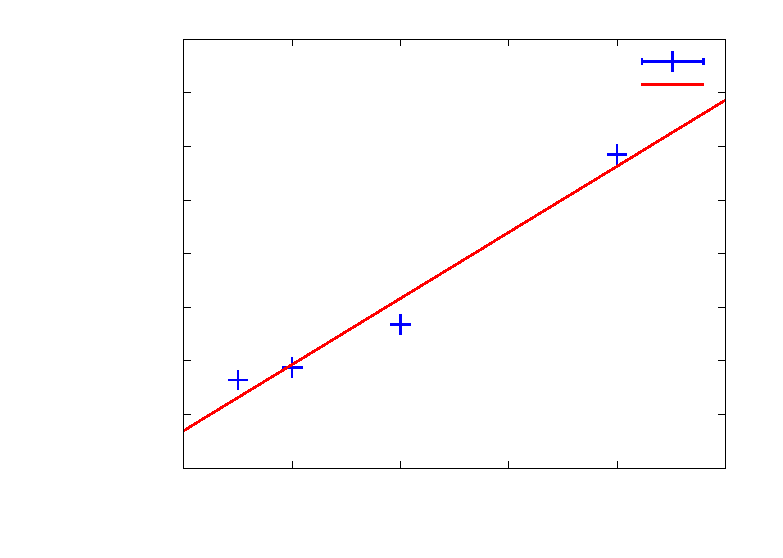
\includegraphics{plots/Relaxivitat_CuT2}}%
    \gplfronttext
  \end{picture}%
\endgroup
}
        \caption{Bestimmung der Relaxivität $r_2$ mit Kupfer als Kontrastmittel. Analog zu Abbildung \ref{fig:RelaxCUT1}.}
        \label{fig:RelaxCUT2}
    \end{subfigure}
    \begin{subfigure}[b]{0.5\textwidth}
        \centering
        \resizebox{1\textwidth}{!}{% GNUPLOT: LaTeX picture with Postscript
\begingroup
  % Encoding inside the plot.  In the header of your document, this encoding
  % should to defined, e.g., by using
  % \usepackage[cp1252,<other encodings>]{inputenc}
  \inputencoding{cp1252}%
  \makeatletter
  \providecommand\color[2][]{%
    \GenericError{(gnuplot) \space\space\space\@spaces}{%
      Package color not loaded in conjunction with
      terminal option `colourtext'%
    }{See the gnuplot documentation for explanation.%
    }{Either use 'blacktext' in gnuplot or load the package
      color.sty in LaTeX.}%
    \renewcommand\color[2][]{}%
  }%
  \providecommand\includegraphics[2][]{%
    \GenericError{(gnuplot) \space\space\space\@spaces}{%
      Package graphicx or graphics not loaded%
    }{See the gnuplot documentation for explanation.%
    }{The gnuplot epslatex terminal needs graphicx.sty or graphics.sty.}%
    \renewcommand\includegraphics[2][]{}%
  }%
  \providecommand\rotatebox[2]{#2}%
  \@ifundefined{ifGPcolor}{%
    \newif\ifGPcolor
    \GPcolorfalse
  }{}%
  \@ifundefined{ifGPblacktext}{%
    \newif\ifGPblacktext
    \GPblacktexttrue
  }{}%
  % define a \g@addto@macro without @ in the name:
  \let\gplgaddtomacro\g@addto@macro
  % define empty templates for all commands taking text:
  \gdef\gplbacktext{}%
  \gdef\gplfronttext{}%
  \makeatother
  \ifGPblacktext
    % no textcolor at all
    \def\colorrgb#1{}%
    \def\colorgray#1{}%
  \else
    % gray or color?
    \ifGPcolor
      \def\colorrgb#1{\color[rgb]{#1}}%
      \def\colorgray#1{\color[gray]{#1}}%
      \expandafter\def\csname LTw\endcsname{\color{white}}%
      \expandafter\def\csname LTb\endcsname{\color{black}}%
      \expandafter\def\csname LTa\endcsname{\color{black}}%
      \expandafter\def\csname LT0\endcsname{\color[rgb]{1,0,0}}%
      \expandafter\def\csname LT1\endcsname{\color[rgb]{0,1,0}}%
      \expandafter\def\csname LT2\endcsname{\color[rgb]{0,0,1}}%
      \expandafter\def\csname LT3\endcsname{\color[rgb]{1,0,1}}%
      \expandafter\def\csname LT4\endcsname{\color[rgb]{0,1,1}}%
      \expandafter\def\csname LT5\endcsname{\color[rgb]{1,1,0}}%
      \expandafter\def\csname LT6\endcsname{\color[rgb]{0,0,0}}%
      \expandafter\def\csname LT7\endcsname{\color[rgb]{1,0.3,0}}%
      \expandafter\def\csname LT8\endcsname{\color[rgb]{0.5,0.5,0.5}}%
    \else
      % gray
      \def\colorrgb#1{\color{black}}%
      \def\colorgray#1{\color[gray]{#1}}%
      \expandafter\def\csname LTw\endcsname{\color{white}}%
      \expandafter\def\csname LTb\endcsname{\color{black}}%
      \expandafter\def\csname LTa\endcsname{\color{black}}%
      \expandafter\def\csname LT0\endcsname{\color{black}}%
      \expandafter\def\csname LT1\endcsname{\color{black}}%
      \expandafter\def\csname LT2\endcsname{\color{black}}%
      \expandafter\def\csname LT3\endcsname{\color{black}}%
      \expandafter\def\csname LT4\endcsname{\color{black}}%
      \expandafter\def\csname LT5\endcsname{\color{black}}%
      \expandafter\def\csname LT6\endcsname{\color{black}}%
      \expandafter\def\csname LT7\endcsname{\color{black}}%
      \expandafter\def\csname LT8\endcsname{\color{black}}%
    \fi
  \fi
    \setlength{\unitlength}{0.0500bp}%
    \ifx\gptboxheight\undefined%
      \newlength{\gptboxheight}%
      \newlength{\gptboxwidth}%
      \newsavebox{\gptboxtext}%
    \fi%
    \setlength{\fboxrule}{0.5pt}%
    \setlength{\fboxsep}{1pt}%
\begin{picture}(7200.00,5040.00)%
    \gplgaddtomacro\gplbacktext{%
      \csname LTb\endcsname%%
      \put(682,704){\makebox(0,0)[r]{\strut{}$0$}}%
      \put(682,1527){\makebox(0,0)[r]{\strut{}$2$}}%
      \put(682,2350){\makebox(0,0)[r]{\strut{}$4$}}%
      \put(682,3173){\makebox(0,0)[r]{\strut{}$6$}}%
      \put(682,3996){\makebox(0,0)[r]{\strut{}$8$}}%
      \put(682,4819){\makebox(0,0)[r]{\strut{}$10$}}%
      \put(814,484){\makebox(0,0){\strut{}$0$}}%
      \put(2012,484){\makebox(0,0){\strut{}$0.1$}}%
      \put(3210,484){\makebox(0,0){\strut{}$0.2$}}%
      \put(4407,484){\makebox(0,0){\strut{}$0.3$}}%
      \put(5605,484){\makebox(0,0){\strut{}$0.4$}}%
      \put(6803,484){\makebox(0,0){\strut{}$0.5$}}%
    }%
    \gplgaddtomacro\gplfronttext{%
      \csname LTb\endcsname%%
      \put(308,2761){\rotatebox{-270}{\makebox(0,0){\strut{}Kehrwert der Zeit in $\si{\frac{1}{\second}}$}}}%
      \put(3808,154){\makebox(0,0){\strut{}Konzentration in  $\si{\frac{\mol}{\meter \tothe{3}}}$}}%
      \csname LTb\endcsname%%
      \put(5858,4606){\makebox(0,0)[r]{\strut{}$1/T_{\text{1}}\left([\ce{Mn^2+}]\right)$}}%
      \csname LTb\endcsname%%
      \put(5858,4386){\makebox(0,0)[r]{\strut{}linearer Fit}}%
    }%
    \gplbacktext
    \put(0,0){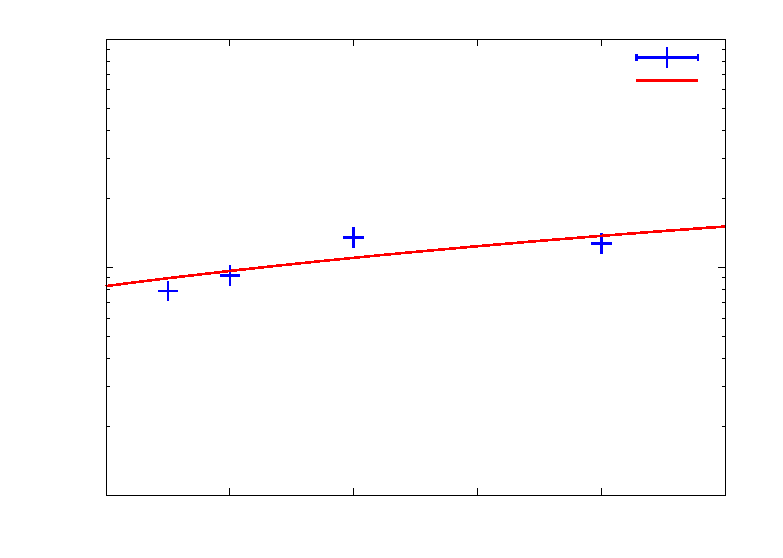
\includegraphics{plots/Relaxivitat_MnT1}}%
    \gplfronttext
  \end{picture}%
\endgroup
}
        \caption{Bestimmung der Relaxivität $r_1$ mit Mangna als Kontrastmittel. Analog zu Abbildung \ref{fig:RelaxCUT1}.}
        \label{fig:RelaxMNT1}
    \end{subfigure}
    \begin{subfigure}[b]{1\textwidth}
        \centering
        \resizebox{0.5\textwidth}{!}{% GNUPLOT: LaTeX picture with Postscript
\begingroup
  % Encoding inside the plot.  In the header of your document, this encoding
  % should to defined, e.g., by using
  % \usepackage[cp1252,<other encodings>]{inputenc}
  \inputencoding{cp1252}%
  \makeatletter
  \providecommand\color[2][]{%
    \GenericError{(gnuplot) \space\space\space\@spaces}{%
      Package color not loaded in conjunction with
      terminal option `colourtext'%
    }{See the gnuplot documentation for explanation.%
    }{Either use 'blacktext' in gnuplot or load the package
      color.sty in LaTeX.}%
    \renewcommand\color[2][]{}%
  }%
  \providecommand\includegraphics[2][]{%
    \GenericError{(gnuplot) \space\space\space\@spaces}{%
      Package graphicx or graphics not loaded%
    }{See the gnuplot documentation for explanation.%
    }{The gnuplot epslatex terminal needs graphicx.sty or graphics.sty.}%
    \renewcommand\includegraphics[2][]{}%
  }%
  \providecommand\rotatebox[2]{#2}%
  \@ifundefined{ifGPcolor}{%
    \newif\ifGPcolor
    \GPcolorfalse
  }{}%
  \@ifundefined{ifGPblacktext}{%
    \newif\ifGPblacktext
    \GPblacktexttrue
  }{}%
  % define a \g@addto@macro without @ in the name:
  \let\gplgaddtomacro\g@addto@macro
  % define empty templates for all commands taking text:
  \gdef\gplbacktext{}%
  \gdef\gplfronttext{}%
  \makeatother
  \ifGPblacktext
    % no textcolor at all
    \def\colorrgb#1{}%
    \def\colorgray#1{}%
  \else
    % gray or color?
    \ifGPcolor
      \def\colorrgb#1{\color[rgb]{#1}}%
      \def\colorgray#1{\color[gray]{#1}}%
      \expandafter\def\csname LTw\endcsname{\color{white}}%
      \expandafter\def\csname LTb\endcsname{\color{black}}%
      \expandafter\def\csname LTa\endcsname{\color{black}}%
      \expandafter\def\csname LT0\endcsname{\color[rgb]{1,0,0}}%
      \expandafter\def\csname LT1\endcsname{\color[rgb]{0,1,0}}%
      \expandafter\def\csname LT2\endcsname{\color[rgb]{0,0,1}}%
      \expandafter\def\csname LT3\endcsname{\color[rgb]{1,0,1}}%
      \expandafter\def\csname LT4\endcsname{\color[rgb]{0,1,1}}%
      \expandafter\def\csname LT5\endcsname{\color[rgb]{1,1,0}}%
      \expandafter\def\csname LT6\endcsname{\color[rgb]{0,0,0}}%
      \expandafter\def\csname LT7\endcsname{\color[rgb]{1,0.3,0}}%
      \expandafter\def\csname LT8\endcsname{\color[rgb]{0.5,0.5,0.5}}%
    \else
      % gray
      \def\colorrgb#1{\color{black}}%
      \def\colorgray#1{\color[gray]{#1}}%
      \expandafter\def\csname LTw\endcsname{\color{white}}%
      \expandafter\def\csname LTb\endcsname{\color{black}}%
      \expandafter\def\csname LTa\endcsname{\color{black}}%
      \expandafter\def\csname LT0\endcsname{\color{black}}%
      \expandafter\def\csname LT1\endcsname{\color{black}}%
      \expandafter\def\csname LT2\endcsname{\color{black}}%
      \expandafter\def\csname LT3\endcsname{\color{black}}%
      \expandafter\def\csname LT4\endcsname{\color{black}}%
      \expandafter\def\csname LT5\endcsname{\color{black}}%
      \expandafter\def\csname LT6\endcsname{\color{black}}%
      \expandafter\def\csname LT7\endcsname{\color{black}}%
      \expandafter\def\csname LT8\endcsname{\color{black}}%
    \fi
  \fi
    \setlength{\unitlength}{0.0500bp}%
    \ifx\gptboxheight\undefined%
      \newlength{\gptboxheight}%
      \newlength{\gptboxwidth}%
      \newsavebox{\gptboxtext}%
    \fi%
    \setlength{\fboxrule}{0.5pt}%
    \setlength{\fboxsep}{1pt}%
\begin{picture}(7200.00,5040.00)%
    \gplgaddtomacro\gplbacktext{%
      \csname LTb\endcsname%%
      \put(1474,704){\makebox(0,0)[r]{\strut{}$0.0*10^{0}$}}%
      \put(1474,1733){\makebox(0,0)[r]{\strut{}$5.0*10^{-3}$}}%
      \put(1474,2762){\makebox(0,0)[r]{\strut{}$1.0*10^{-2}$}}%
      \put(1474,3790){\makebox(0,0)[r]{\strut{}$1.5*10^{-2}$}}%
      \put(1474,4819){\makebox(0,0)[r]{\strut{}$2.0*10^{-2}$}}%
      \put(1606,484){\makebox(0,0){\strut{}$0$}}%
      \put(2645,484){\makebox(0,0){\strut{}$0.1$}}%
      \put(3685,484){\makebox(0,0){\strut{}$0.2$}}%
      \put(4724,484){\makebox(0,0){\strut{}$0.3$}}%
      \put(5764,484){\makebox(0,0){\strut{}$0.4$}}%
      \put(6803,484){\makebox(0,0){\strut{}$0.5$}}%
    }%
    \gplgaddtomacro\gplfronttext{%
      \csname LTb\endcsname%%
      \put(308,2761){\rotatebox{-270}{\makebox(0,0){\strut{}Kehrwert der Zeit in $\si{\per \second}$}}}%
      \put(4204,154){\makebox(0,0){\strut{}Konzentration in  $\si{\mol \per \meter \tothe{3} }$}}%
      \csname LTb\endcsname%%
      \put(5870,4606){\makebox(0,0)[r]{\strut{}$1/T_{\text{2}}\left([\ce{Mn^2+}]\right)$}}%
      \csname LTb\endcsname%%
      \put(5870,4386){\makebox(0,0)[r]{\strut{}linearer Fit}}%
    }%
    \gplbacktext
    \put(0,0){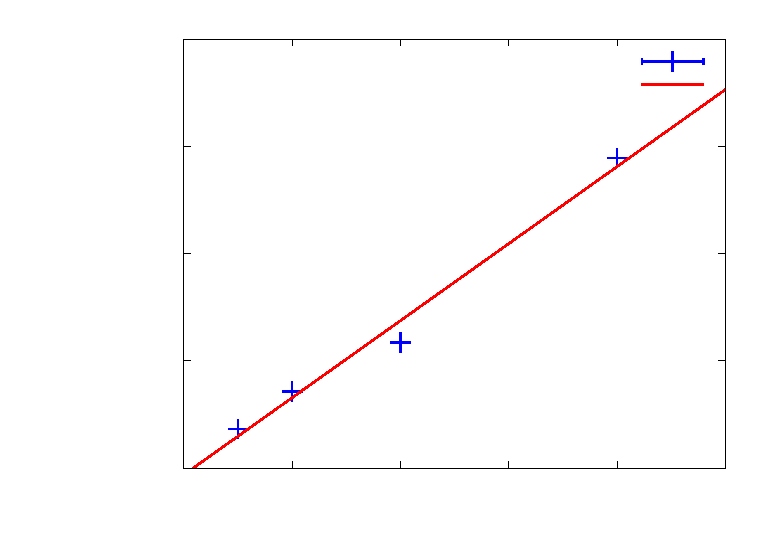
\includegraphics{plots/Relaxivitat_MnT2}}%
    \gplfronttext
  \end{picture}%
\endgroup
}
        \caption{Bestimmung der Relaxivität $r_2$ mit Mangan als Kontrastmittel. Analog zu Abbildung \ref{fig:RelaxCUT1}.}
        \label{fig:RelaxMNT2}
    \end{subfigure}
    \caption{Übersicht über alle ermittelten Relaxivitäten.}
    \label{fig:RelaxAlle}
\end{figure}




\begin{figure}[H]
    \begin{subfigure}[b]{0.5\textwidth}
        \centering
        \resizebox{1\textwidth}{!}{% GNUPLOT: LaTeX picture with Postscript
\begingroup
  % Encoding inside the plot.  In the header of your document, this encoding
  % should to defined, e.g., by using
  % \usepackage[cp1252,<other encodings>]{inputenc}
  \inputencoding{cp1252}%
  \makeatletter
  \providecommand\color[2][]{%
    \GenericError{(gnuplot) \space\space\space\@spaces}{%
      Package color not loaded in conjunction with
      terminal option `colourtext'%
    }{See the gnuplot documentation for explanation.%
    }{Either use 'blacktext' in gnuplot or load the package
      color.sty in LaTeX.}%
    \renewcommand\color[2][]{}%
  }%
  \providecommand\includegraphics[2][]{%
    \GenericError{(gnuplot) \space\space\space\@spaces}{%
      Package graphicx or graphics not loaded%
    }{See the gnuplot documentation for explanation.%
    }{The gnuplot epslatex terminal needs graphicx.sty or graphics.sty.}%
    \renewcommand\includegraphics[2][]{}%
  }%
  \providecommand\rotatebox[2]{#2}%
  \@ifundefined{ifGPcolor}{%
    \newif\ifGPcolor
    \GPcolorfalse
  }{}%
  \@ifundefined{ifGPblacktext}{%
    \newif\ifGPblacktext
    \GPblacktexttrue
  }{}%
  % define a \g@addto@macro without @ in the name:
  \let\gplgaddtomacro\g@addto@macro
  % define empty templates for all commands taking text:
  \gdef\gplbacktext{}%
  \gdef\gplfronttext{}%
  \makeatother
  \ifGPblacktext
    % no textcolor at all
    \def\colorrgb#1{}%
    \def\colorgray#1{}%
  \else
    % gray or color?
    \ifGPcolor
      \def\colorrgb#1{\color[rgb]{#1}}%
      \def\colorgray#1{\color[gray]{#1}}%
      \expandafter\def\csname LTw\endcsname{\color{white}}%
      \expandafter\def\csname LTb\endcsname{\color{black}}%
      \expandafter\def\csname LTa\endcsname{\color{black}}%
      \expandafter\def\csname LT0\endcsname{\color[rgb]{1,0,0}}%
      \expandafter\def\csname LT1\endcsname{\color[rgb]{0,1,0}}%
      \expandafter\def\csname LT2\endcsname{\color[rgb]{0,0,1}}%
      \expandafter\def\csname LT3\endcsname{\color[rgb]{1,0,1}}%
      \expandafter\def\csname LT4\endcsname{\color[rgb]{0,1,1}}%
      \expandafter\def\csname LT5\endcsname{\color[rgb]{1,1,0}}%
      \expandafter\def\csname LT6\endcsname{\color[rgb]{0,0,0}}%
      \expandafter\def\csname LT7\endcsname{\color[rgb]{1,0.3,0}}%
      \expandafter\def\csname LT8\endcsname{\color[rgb]{0.5,0.5,0.5}}%
    \else
      % gray
      \def\colorrgb#1{\color{black}}%
      \def\colorgray#1{\color[gray]{#1}}%
      \expandafter\def\csname LTw\endcsname{\color{white}}%
      \expandafter\def\csname LTb\endcsname{\color{black}}%
      \expandafter\def\csname LTa\endcsname{\color{black}}%
      \expandafter\def\csname LT0\endcsname{\color{black}}%
      \expandafter\def\csname LT1\endcsname{\color{black}}%
      \expandafter\def\csname LT2\endcsname{\color{black}}%
      \expandafter\def\csname LT3\endcsname{\color{black}}%
      \expandafter\def\csname LT4\endcsname{\color{black}}%
      \expandafter\def\csname LT5\endcsname{\color{black}}%
      \expandafter\def\csname LT6\endcsname{\color{black}}%
      \expandafter\def\csname LT7\endcsname{\color{black}}%
      \expandafter\def\csname LT8\endcsname{\color{black}}%
    \fi
  \fi
    \setlength{\unitlength}{0.0500bp}%
    \ifx\gptboxheight\undefined%
      \newlength{\gptboxheight}%
      \newlength{\gptboxwidth}%
      \newsavebox{\gptboxtext}%
    \fi%
    \setlength{\fboxrule}{0.5pt}%
    \setlength{\fboxsep}{1pt}%
\begin{picture}(7200.00,5040.00)%
    \gplgaddtomacro\gplbacktext{%
      \csname LTb\endcsname%%
      \put(814,704){\makebox(0,0)[r]{\strut{}$0$}}%
      \put(814,1527){\makebox(0,0)[r]{\strut{}$0.2$}}%
      \put(814,2350){\makebox(0,0)[r]{\strut{}$0.4$}}%
      \put(814,3173){\makebox(0,0)[r]{\strut{}$0.6$}}%
      \put(814,3996){\makebox(0,0)[r]{\strut{}$0.8$}}%
      \put(814,4819){\makebox(0,0)[r]{\strut{}$1$}}%
      \put(946,484){\makebox(0,0){\strut{}$0$}}%
      \put(1922,484){\makebox(0,0){\strut{}$1000$}}%
      \put(2898,484){\makebox(0,0){\strut{}$2000$}}%
      \put(3875,484){\makebox(0,0){\strut{}$3000$}}%
      \put(4851,484){\makebox(0,0){\strut{}$4000$}}%
      \put(5827,484){\makebox(0,0){\strut{}$5000$}}%
      \put(6803,484){\makebox(0,0){\strut{}$6000$}}%
    }%
    \gplgaddtomacro\gplfronttext{%
      \csname LTb\endcsname%%
      \put(308,2761){\rotatebox{-270}{\makebox(0,0){\strut{}D\"ampfung $\frac{\text{E}}{\text{E}_0}$}}}%
      \put(3874,154){\makebox(0,0){\strut{}Zeit in $\si{\milli \second}$}}%
      \csname LTb\endcsname%%
      \put(5860,4606){\makebox(0,0)[r]{\strut{}$Cu^{2+} \SI{250}{\micro\mole}$}}%
      \csname LTb\endcsname%%
      \put(5860,4386){\makebox(0,0)[r]{\strut{}$Cu^{2+} \SI{1000}{\micro\mole}$}}%
      \csname LTb\endcsname%%
      \put(5860,4166){\makebox(0,0)[r]{\strut{}$Cu^{2+} \SI{250}{\micro\mole}$}}%
      \csname LTb\endcsname%%
      \put(5860,3946){\makebox(0,0)[r]{\strut{}$Cu^{2+} \SI{2000}{\micro\mole}$}}%
      \csname LTb\endcsname%%
      \put(5860,3726){\makebox(0,0)[r]{\strut{}Wasser}}%
    }%
    \gplbacktext
    \put(0,0){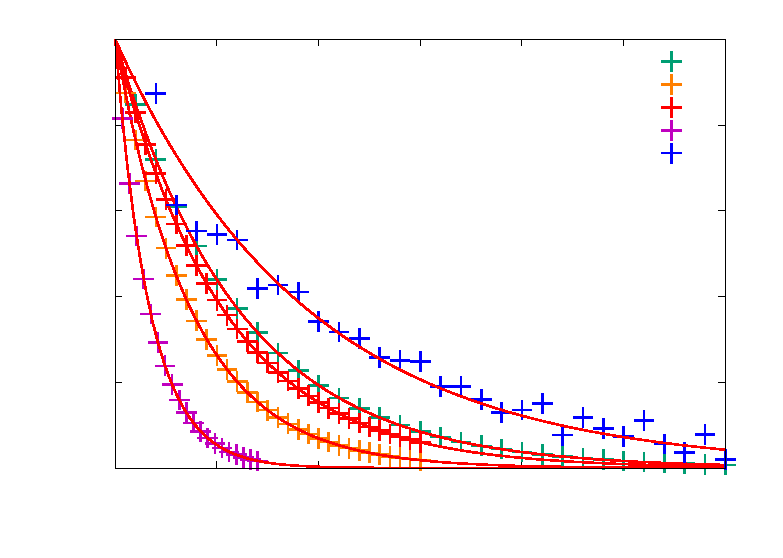
\includegraphics{plots/KupferalleT2}}%
    \gplfronttext
  \end{picture}%
\endgroup
}
        \caption{Alle $T_2$-Messungen aller verwendeten Kupferkonzentrationen.}
        \label{fig:T2CU}
    \end{subfigure}
    \begin{subfigure}[b]{0.5\textwidth}
        \centering
        \resizebox{1\textwidth}{!}{% GNUPLOT: LaTeX picture with Postscript
\begingroup
  % Encoding inside the plot.  In the header of your document, this encoding
  % should to defined, e.g., by using
  % \usepackage[cp1252,<other encodings>]{inputenc}
  \inputencoding{cp1252}%
  \makeatletter
  \providecommand\color[2][]{%
    \GenericError{(gnuplot) \space\space\space\@spaces}{%
      Package color not loaded in conjunction with
      terminal option `colourtext'%
    }{See the gnuplot documentation for explanation.%
    }{Either use 'blacktext' in gnuplot or load the package
      color.sty in LaTeX.}%
    \renewcommand\color[2][]{}%
  }%
  \providecommand\includegraphics[2][]{%
    \GenericError{(gnuplot) \space\space\space\@spaces}{%
      Package graphicx or graphics not loaded%
    }{See the gnuplot documentation for explanation.%
    }{The gnuplot epslatex terminal needs graphicx.sty or graphics.sty.}%
    \renewcommand\includegraphics[2][]{}%
  }%
  \providecommand\rotatebox[2]{#2}%
  \@ifundefined{ifGPcolor}{%
    \newif\ifGPcolor
    \GPcolorfalse
  }{}%
  \@ifundefined{ifGPblacktext}{%
    \newif\ifGPblacktext
    \GPblacktexttrue
  }{}%
  % define a \g@addto@macro without @ in the name:
  \let\gplgaddtomacro\g@addto@macro
  % define empty templates for all commands taking text:
  \gdef\gplbacktext{}%
  \gdef\gplfronttext{}%
  \makeatother
  \ifGPblacktext
    % no textcolor at all
    \def\colorrgb#1{}%
    \def\colorgray#1{}%
  \else
    % gray or color?
    \ifGPcolor
      \def\colorrgb#1{\color[rgb]{#1}}%
      \def\colorgray#1{\color[gray]{#1}}%
      \expandafter\def\csname LTw\endcsname{\color{white}}%
      \expandafter\def\csname LTb\endcsname{\color{black}}%
      \expandafter\def\csname LTa\endcsname{\color{black}}%
      \expandafter\def\csname LT0\endcsname{\color[rgb]{1,0,0}}%
      \expandafter\def\csname LT1\endcsname{\color[rgb]{0,1,0}}%
      \expandafter\def\csname LT2\endcsname{\color[rgb]{0,0,1}}%
      \expandafter\def\csname LT3\endcsname{\color[rgb]{1,0,1}}%
      \expandafter\def\csname LT4\endcsname{\color[rgb]{0,1,1}}%
      \expandafter\def\csname LT5\endcsname{\color[rgb]{1,1,0}}%
      \expandafter\def\csname LT6\endcsname{\color[rgb]{0,0,0}}%
      \expandafter\def\csname LT7\endcsname{\color[rgb]{1,0.3,0}}%
      \expandafter\def\csname LT8\endcsname{\color[rgb]{0.5,0.5,0.5}}%
    \else
      % gray
      \def\colorrgb#1{\color{black}}%
      \def\colorgray#1{\color[gray]{#1}}%
      \expandafter\def\csname LTw\endcsname{\color{white}}%
      \expandafter\def\csname LTb\endcsname{\color{black}}%
      \expandafter\def\csname LTa\endcsname{\color{black}}%
      \expandafter\def\csname LT0\endcsname{\color{black}}%
      \expandafter\def\csname LT1\endcsname{\color{black}}%
      \expandafter\def\csname LT2\endcsname{\color{black}}%
      \expandafter\def\csname LT3\endcsname{\color{black}}%
      \expandafter\def\csname LT4\endcsname{\color{black}}%
      \expandafter\def\csname LT5\endcsname{\color{black}}%
      \expandafter\def\csname LT6\endcsname{\color{black}}%
      \expandafter\def\csname LT7\endcsname{\color{black}}%
      \expandafter\def\csname LT8\endcsname{\color{black}}%
    \fi
  \fi
    \setlength{\unitlength}{0.0500bp}%
    \ifx\gptboxheight\undefined%
      \newlength{\gptboxheight}%
      \newlength{\gptboxwidth}%
      \newsavebox{\gptboxtext}%
    \fi%
    \setlength{\fboxrule}{0.5pt}%
    \setlength{\fboxsep}{1pt}%
\begin{picture}(7200.00,5040.00)%
    \gplgaddtomacro\gplbacktext{%
      \csname LTb\endcsname%%
      \put(814,704){\makebox(0,0)[r]{\strut{}$0$}}%
      \put(814,1527){\makebox(0,0)[r]{\strut{}$0.2$}}%
      \put(814,2350){\makebox(0,0)[r]{\strut{}$0.4$}}%
      \put(814,3173){\makebox(0,0)[r]{\strut{}$0.6$}}%
      \put(814,3996){\makebox(0,0)[r]{\strut{}$0.8$}}%
      \put(814,4819){\makebox(0,0)[r]{\strut{}$1$}}%
      \put(946,484){\makebox(0,0){\strut{}$0$}}%
      \put(1922,484){\makebox(0,0){\strut{}$1000$}}%
      \put(2898,484){\makebox(0,0){\strut{}$2000$}}%
      \put(3875,484){\makebox(0,0){\strut{}$3000$}}%
      \put(4851,484){\makebox(0,0){\strut{}$4000$}}%
      \put(5827,484){\makebox(0,0){\strut{}$5000$}}%
      \put(6803,484){\makebox(0,0){\strut{}$6000$}}%
    }%
    \gplgaddtomacro\gplfronttext{%
      \csname LTb\endcsname%%
      \put(198,2761){\rotatebox{-270}{\makebox(0,0){\strut{}D\"ampfung $\frac{\text{E}}{\text{E}_0}$}}}%
      \put(3874,154){\makebox(0,0){\strut{}Zeit in $\si{\milli \second}$}}%
      \csname LTb\endcsname%%
      \put(5860,3680){\makebox(0,0)[r]{\strut{}$Mn^{2+} \SI{25}{\micro\mole}$}}%
      \csname LTb\endcsname%%
      \put(5860,3460){\makebox(0,0)[r]{\strut{}$Mn^{2+} \SI{50}{\micro\mole}$}}%
      \csname LTb\endcsname%%
      \put(5860,3240){\makebox(0,0)[r]{\strut{}$Mn^{2+} \SI{100}{\micro\mole}$}}%
      \csname LTb\endcsname%%
      \put(5860,3020){\makebox(0,0)[r]{\strut{}$Mn^{2+} \SI{200}{\micro\mole}$}}%
      \csname LTb\endcsname%%
      \put(5860,2800){\makebox(0,0)[r]{\strut{}Wasser}}%
    }%
    \gplbacktext
    \put(0,0){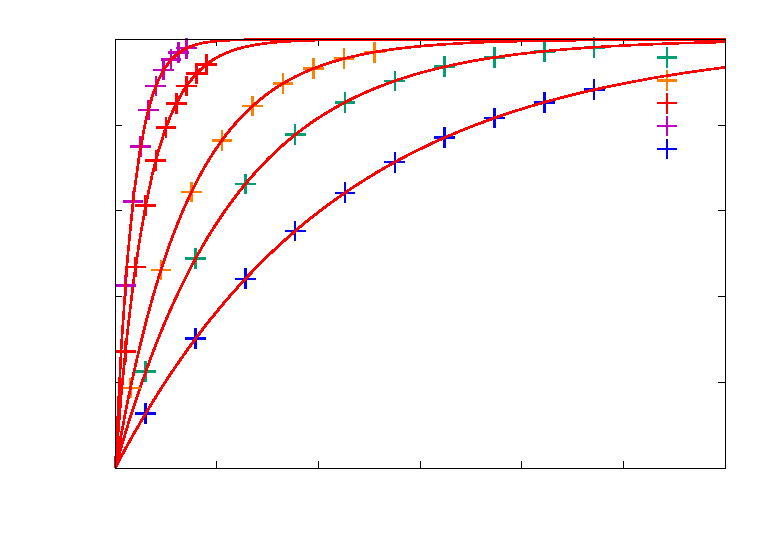
\includegraphics{plots/ManganalleT1}}%
    \gplfronttext
  \end{picture}%
\endgroup
}
        \caption{Alle $T_1$-Messungen aller verwendeten Mangankonzentrationen.}
        \label{fig:T1Mn}
    \end{subfigure}
    \begin{subfigure}[b]{1\textwidth}
        \centering
        \resizebox{0.5\textwidth}{!}{% GNUPLOT: LaTeX picture with Postscript
\begingroup
  % Encoding inside the plot.  In the header of your document, this encoding
  % should to defined, e.g., by using
  % \usepackage[cp1252,<other encodings>]{inputenc}
  \inputencoding{cp1252}%
  \makeatletter
  \providecommand\color[2][]{%
    \GenericError{(gnuplot) \space\space\space\@spaces}{%
      Package color not loaded in conjunction with
      terminal option `colourtext'%
    }{See the gnuplot documentation for explanation.%
    }{Either use 'blacktext' in gnuplot or load the package
      color.sty in LaTeX.}%
    \renewcommand\color[2][]{}%
  }%
  \providecommand\includegraphics[2][]{%
    \GenericError{(gnuplot) \space\space\space\@spaces}{%
      Package graphicx or graphics not loaded%
    }{See the gnuplot documentation for explanation.%
    }{The gnuplot epslatex terminal needs graphicx.sty or graphics.sty.}%
    \renewcommand\includegraphics[2][]{}%
  }%
  \providecommand\rotatebox[2]{#2}%
  \@ifundefined{ifGPcolor}{%
    \newif\ifGPcolor
    \GPcolorfalse
  }{}%
  \@ifundefined{ifGPblacktext}{%
    \newif\ifGPblacktext
    \GPblacktexttrue
  }{}%
  % define a \g@addto@macro without @ in the name:
  \let\gplgaddtomacro\g@addto@macro
  % define empty templates for all commands taking text:
  \gdef\gplbacktext{}%
  \gdef\gplfronttext{}%
  \makeatother
  \ifGPblacktext
    % no textcolor at all
    \def\colorrgb#1{}%
    \def\colorgray#1{}%
  \else
    % gray or color?
    \ifGPcolor
      \def\colorrgb#1{\color[rgb]{#1}}%
      \def\colorgray#1{\color[gray]{#1}}%
      \expandafter\def\csname LTw\endcsname{\color{white}}%
      \expandafter\def\csname LTb\endcsname{\color{black}}%
      \expandafter\def\csname LTa\endcsname{\color{black}}%
      \expandafter\def\csname LT0\endcsname{\color[rgb]{1,0,0}}%
      \expandafter\def\csname LT1\endcsname{\color[rgb]{0,1,0}}%
      \expandafter\def\csname LT2\endcsname{\color[rgb]{0,0,1}}%
      \expandafter\def\csname LT3\endcsname{\color[rgb]{1,0,1}}%
      \expandafter\def\csname LT4\endcsname{\color[rgb]{0,1,1}}%
      \expandafter\def\csname LT5\endcsname{\color[rgb]{1,1,0}}%
      \expandafter\def\csname LT6\endcsname{\color[rgb]{0,0,0}}%
      \expandafter\def\csname LT7\endcsname{\color[rgb]{1,0.3,0}}%
      \expandafter\def\csname LT8\endcsname{\color[rgb]{0.5,0.5,0.5}}%
    \else
      % gray
      \def\colorrgb#1{\color{black}}%
      \def\colorgray#1{\color[gray]{#1}}%
      \expandafter\def\csname LTw\endcsname{\color{white}}%
      \expandafter\def\csname LTb\endcsname{\color{black}}%
      \expandafter\def\csname LTa\endcsname{\color{black}}%
      \expandafter\def\csname LT0\endcsname{\color{black}}%
      \expandafter\def\csname LT1\endcsname{\color{black}}%
      \expandafter\def\csname LT2\endcsname{\color{black}}%
      \expandafter\def\csname LT3\endcsname{\color{black}}%
      \expandafter\def\csname LT4\endcsname{\color{black}}%
      \expandafter\def\csname LT5\endcsname{\color{black}}%
      \expandafter\def\csname LT6\endcsname{\color{black}}%
      \expandafter\def\csname LT7\endcsname{\color{black}}%
      \expandafter\def\csname LT8\endcsname{\color{black}}%
    \fi
  \fi
    \setlength{\unitlength}{0.0500bp}%
    \ifx\gptboxheight\undefined%
      \newlength{\gptboxheight}%
      \newlength{\gptboxwidth}%
      \newsavebox{\gptboxtext}%
    \fi%
    \setlength{\fboxrule}{0.5pt}%
    \setlength{\fboxsep}{1pt}%
\begin{picture}(7200.00,5040.00)%
    \gplgaddtomacro\gplbacktext{%
      \csname LTb\endcsname%%
      \put(814,704){\makebox(0,0)[r]{\strut{}$0$}}%
      \put(814,1527){\makebox(0,0)[r]{\strut{}$0.2$}}%
      \put(814,2350){\makebox(0,0)[r]{\strut{}$0.4$}}%
      \put(814,3173){\makebox(0,0)[r]{\strut{}$0.6$}}%
      \put(814,3996){\makebox(0,0)[r]{\strut{}$0.8$}}%
      \put(814,4819){\makebox(0,0)[r]{\strut{}$1$}}%
      \put(946,484){\makebox(0,0){\strut{}$0$}}%
      \put(1922,484){\makebox(0,0){\strut{}$1000$}}%
      \put(2898,484){\makebox(0,0){\strut{}$2000$}}%
      \put(3875,484){\makebox(0,0){\strut{}$3000$}}%
      \put(4851,484){\makebox(0,0){\strut{}$4000$}}%
      \put(5827,484){\makebox(0,0){\strut{}$5000$}}%
      \put(6803,484){\makebox(0,0){\strut{}$6000$}}%
    }%
    \gplgaddtomacro\gplfronttext{%
      \csname LTb\endcsname%%
      \put(198,2761){\rotatebox{-270}{\makebox(0,0){\strut{}D\"ampfung $\frac{\text{E}}{\text{E}_0}$}}}%
      \put(3874,154){\makebox(0,0){\strut{}Zeit in $\si{\milli \second}$}}%
      \csname LTb\endcsname%%
      \put(5860,4606){\makebox(0,0)[r]{\strut{}$Mn^{2+} \SI{25}{\micro\mole}$}}%
      \csname LTb\endcsname%%
      \put(5860,4386){\makebox(0,0)[r]{\strut{}$Mn^{2+} \SI{100}{\micro\mole}$}}%
      \csname LTb\endcsname%%
      \put(5860,4166){\makebox(0,0)[r]{\strut{}$Mn^{2+} \SI{25}{\micro\mole}$}}%
      \csname LTb\endcsname%%
      \put(5860,3946){\makebox(0,0)[r]{\strut{}$Mn^{2+} \SI{200}{\micro\mole}$}}%
      \csname LTb\endcsname%%
      \put(5860,3726){\makebox(0,0)[r]{\strut{}Wasser}}%
    }%
    \gplbacktext
    \put(0,0){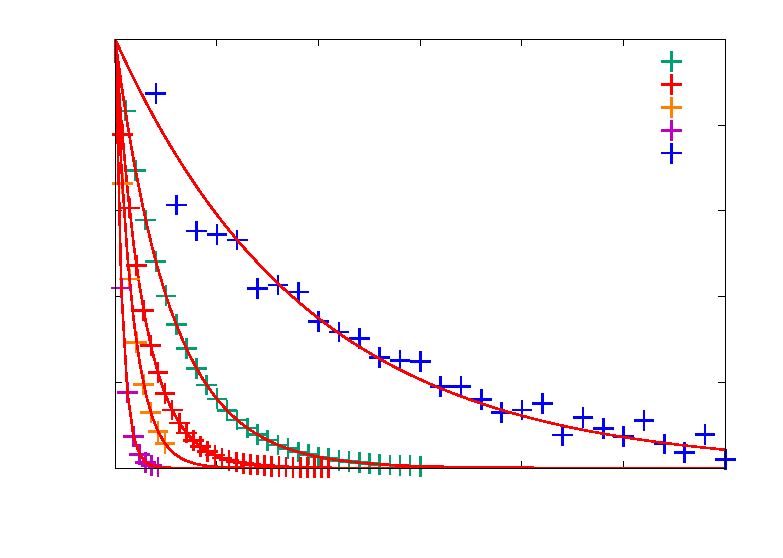
\includegraphics{plots/ManganalleT2}}%
    \gplfronttext
  \end{picture}%
\endgroup
}
        \caption{Alle $T_2$-Messungen aller verwendeten Mangankonzentrationen.}
        \label{fig:T2Mn}
    \end{subfigure}
    \caption{Übersicht über alle $T_1$- und $T_2$-Messungen für beide verwendeten Kontrastmittel mit jeweils unterschiedlichen Konzentrationen.}
    \label{fig:RelaxZeitAlle}
\end{figure}
